\documentclass[11pt,a4paper]{report}
\usepackage[utf8]{inputenc}
\usepackage{amsmath}
\usepackage{amsfonts}
\usepackage{amssymb}
\usepackage[utf8]{inputenc}
\usepackage[T1]{fontenc}
\usepackage{textcomp}
\usepackage{gensymb}
\usepackage{graphicx}
\usepackage{epstopdf}
\begin{document}

\begin{titlepage}

\newcommand{\HRule}{\rule{\linewidth}{0.5mm}} % Defines a new command for the horizontal lines, change thickness here

\center % Center everything on the page
 
%----------------------------------------------------------------------------------------
%	HEADING SECTIONS
%----------------------------------------------------------------------------------------

\textsc{\LARGE Utrecht University}\\[1.5cm] % Name of your university/college
\textsc{\Large Master Thesis Project}\\[0.5cm] % Major heading such as course name
\textsc{\large Minor Heading}\\[0.5cm] % Minor heading such as course title

%----------------------------------------------------------------------------------------
%	TITLE SECTION
%----------------------------------------------------------------------------------------

\HRule \\[0.4cm]
{ \huge \bfseries Hair Rendering: Importance Sampling of Dual Scattering Approximation}\\[0.4cm] % Title of your document
\HRule \\[1.5cm]
 
%----------------------------------------------------------------------------------------
%	AUTHOR SECTION
%----------------------------------------------------------------------------------------

\begin{minipage}{0.4\textwidth}
\begin{flushleft} \large
\emph{Author:}\\
Jeffrey \textsc{Lemein}% Your name
\end{flushleft}
\end{minipage}
~
\begin{minipage}{0.4\textwidth}
\begin{flushright} \large
\emph{Supervisor:} \\
Prof. Remco \textsc{Veltkamp} \\ % Supervisor's Name
Dr. Robby T. \textsc{Tan} \\ % Supervisor's Name
Desmond \textsc{Chik} \\ % Supervisor's Name \\
Daniel \textsc{Heckenberg}  % Supervisor's Name \\
\end{flushright}
\end{minipage}\\[4cm]

% If you don't want a supervisor, uncomment the two lines below and remove the section above
%\Large \emph{Author:}\\
%John \textsc{Smith}\\[3cm] % Your name

%----------------------------------------------------------------------------------------
%	DATE SECTION
%----------------------------------------------------------------------------------------

{\large \today}\\[3cm] % Date, change the \today to a set date if you want to be precise

%----------------------------------------------------------------------------------------
%	LOGO SECTION
%----------------------------------------------------------------------------------------

%\includegraphics{Logo}\\[1cm] % Include a department/university logo - this will require the graphicx package
 
%----------------------------------------------------------------------------------------

\vfill % Fill the rest of the page with whitespace

\end{titlepage}

%----------------------------------------------------------------------------
% Standard thesis layout:
%
% 1. Title page: including student name, student number, supervisor names, and date
% 2. Abstract
% 3. Acknowledgement (optional)
% 4. Chapter 1: Introduction
% 5. Chapter 2: Related work / Background Knowledge
% 6. Chapter 3: Theory
% 7. Chapter 4: Experimental Results and Evaluation
% 8. Chapter 5: Conclusion
% 9. Appendix (optional)
% 10. References
%
\begin{abstract}
Your abstract goes here...
...
\end{abstract}

%
% ===============================================================================
%
\tableofcontents

\chapter{Introduction}

% a. State the background of the field, why it is interesting, what the possible applications are.

Hair rendering has always been a challenging task due to the amount of hair strands and the complex scattering behaviour. A lot of work has been put into approximating the appearance of a hair volume. For example by applying transparent textures to a bounding volume. Since a couple of years there is a shift towards physically based rendering using ray tracing. This is partly made possible by faster hardware, but also because of interest in realistic renderings. Theories have been devised to increase rendering speeds such as Monte-Carlo sampling in combination with importance sampling.

Hair rendering becomes increasingly more realistic and having realistic hair models is primarily important for the following applications:

\begin{itemize}
\item Animation movie industry: to efficiently render realistic hair, instead of simplified models.
\item Game industry to enhance realism and for better visual effects.
\item Clothes manufacturers: to be able to realistically render custom fabrics and see what the visual appearance of the fiber structure will look like under different lighting conditions.
\item Hair styling industry: to realistically render the appearance of hair styling products applied to the hair.
\end{itemize}

There are a bunch of applications for hair rendering. Efficient and realistic hair rendering algorithms will benefit realism in computer animation. 

Possible applications are mainly in the field of computer graphics. Animation studios can enhance their models

Hair rendering on the fiber level can also be applied to clothes manufacturers to see how specific materials may affect the visual appearance of the clothing.



\section{Existing methods}

% d. State what the applications if you can achieve the goal
% f. State the scope (namely, assumptions or the constraints) of the solutions.
% g. Optional: the organization of the remaining chapter.

% c. State why existing methods cannot solve the problems
Hair rendering using the Kajiya and Kay model falls short of realism. The Marschner model improves the model considerably by using measured observations. The dual scattering approximation extends the Marschner model by taking into account scattering behaviour for multiple fibers, instead of just single-fiber scattering. It does this by presenting an efficient shader-based algorithm. Since physically-based rendering becomes more important these years, we need to implement an efficient sampling framework for the dual scattering approximation.

\section{Goal and approach}
% b. State your goal (what problems you really want to solve)
In this thesis project the goal is to extend the dual scattering approximation model with importance sampling. Importance sampling is a variance reduction technique. I will focus on a couple of parameters when finding an importance sampling function. These parameters are the eccentricity and the number of hair strands. Other parameters are assumed to be constant, such as the index of refraction of 1.55, which is a completely logical value for human hair strands. This means that the importance sampling function might be less efficient for hair strands with a different index of refraction.

% e. State how you want to approach the problem
To find a sampling strategy plots will be made to show the response of the dual scattering approximation for different eccentricity values and number of occluded strands. These occluded strands are the number of strands that are covered between a point to render and the light source. More occluded strands mean that less light will reach the point in question. The response graphs are to be matched with a mathematical formula that can be inverted to a cumulative distribution form (CDF). This is necessary for efficient importance sampling. Speed gains or variance decrease tests are performed afterwards to show the performance of the importance sampling function.



%
% ===============================================================================
%

\chapter{Background}


\chapter{Related Work}

% a. Discuss the existing methods and state why they cannot solve the problems or achieve the goal entirely.
% b. Discuss other related work or knowledge that is necessary to understand the theory explained in Chapter 3.
% c. Ask yourself if the information will be sufficient if a student who is new in the field reads this chapter.


\section{Hair Characteristics}

There are different kind of hair styles. According to Ward et al.~\cite{ward} hair can be smooth, jagged, wavy or curly depending on the ethnic group. Three different ethnic groups are distinguished: Asian, African and Caucasian hair. A hair fiber can either have a circular or elliptical cross section. Asian hair tends to be very smooth and regular with a circular cross section, whereas African hair is very irregular and has an elliptical cross section. Caucasian hair is in between and can be a mixture of both properties.

The follicle is the active part of hair under the skin and produces keratin proteins that compose the hair material~\cite{hadap}. The visible part of the hair is called the hair shaft. Hair has almost uniform cross section, natural twist and natural curvatures all along~\cite{hadap}. It makes the hair appear curly, straight, fuzzy, smooth, etcetera. These parameters are characteristic for the ethnic group.

A hair fiber of the human scalp consist of three layers. The outside layer is the cuticle. The cuticle is a thin sheath of protective layers that surround the inner cortex. It forms the interface between the fiber and the air. The protective sheath consist of flat cells on top of each other. Because of the overlapped arrangement the surface normal is tilted slightly from the overall normal of the fiber's surface. According to Marschner et al.~\cite{marschner} the surface normals are tiled by approximately 3 degrees toward the root. See figure~\ref{fig_hair_structure} for a view on the cuticle scales.

The center of the hair fiber consists of the medulla: a pigmented core. The pigments give hair its color. The cortex is the core of the fiber and provides the strength for the hair fiber. The cortex is filled with keratin, contributing 90\% of the total weight~\cite{ward}. Keratin is a stiff material that causes hair to be easily bend and twisted, but hard to shear and stretch.

Hair consists of amorphous proteins that act as a transparent medium with an index of refraction of $\eta = 1.55$~\cite{ward}. A hair model will later be introduced that models hair fibers as dielectric cylinders where the index of refraction is important in deciding the refraction angle and the amount of Fresnel reflection.

\begin{figure}[h]
\begin{center}
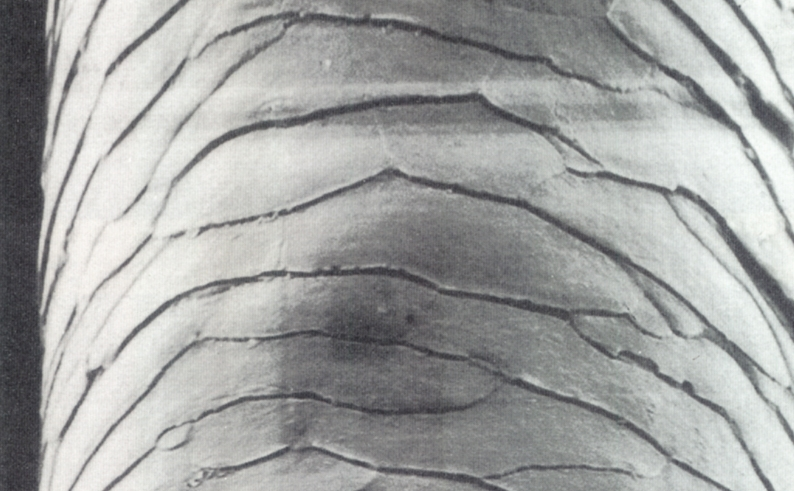
\includegraphics[scale=0.4]{images/hair_structure.jpeg}
\caption{The tilted cuticle scales on the outside of the hair fiber.}
\label{fig_hair_structure}
\end{center}
\end{figure}

\section{Radiometry}
It is important to understand the terminology in radiometry to get a good understanding of the theory that is explained in this report. If you are already familiar to this theory, you can skip this section. This theory is primarily meant for ones that are new to the field of rendering. 

\subsection{Power and radiant flux}

Power is the rate at which energy is transferred and is expressed in watts (W). A single watt describes the transfer of a single Joule (J) of energy per unit time (s).

A lot of electronic machines consume power, and each one does it in it's own particular way. You can think of light, heat, force, pressure, etcetera. Consider a light source that emits light particles through the scene at a certain rate. Some lights are stronger than others, meaning that the stronger light has more power and sends out the energy at a faster rate into the scene. These elementary light particles are called photons. Photons exhibit a wave-particle duality. On one side they can be treated as minuscule particles and on the other side they can be treated as waves, or more specifically: electromagnetic waves.

The rate at which a light source sends out electromagnetic waves is called radiant flux. Radiant flux $\Phi$ is the power of electromagnetic waves and describes the transfer of radiant energy (J) per unit time (s). Radiant flux is therefore also expressed in watts (W).

\subsection{Solid Angle and Radiant Intensity}

A two-dimensional angle can be thought of as drawing two lines from the center of a circle outward. Angle are represented as degrees or radians, but radians are more convenient for mathematical purposes. A solid angle $\Omega$ is the two-dimensional angle in three dimensional space that an object subtends at a point. Consider projecting an object on a unit sphere. An object that is closer to the sphere may have the same solid angle as an object that is farther away. In this case, the object that is farther away must be bigger in shape. A solid angle is a dimensionless unit of measurement called a steradian ($sr$). Steradian coming from squared radian.

The picture below clearly shows the difference.

[TODO: place image]\\

The radiant intensity $I$ is a measure of the intensity of electromagnetic radiation. It can be seen as the energy flow divided by the solid angle in which it is transmitted. Radiant intensity is defined as radiant power per unit solid angle ($W \cdot sr^{-1}$).

\subsection{Radiance versus Irradiance}

Formally, irradiance $E$ is defined as the amount of power of electromagnetic radiation per unit area incident on a surface. The unit for irradiance is watts per square meter ($W \cdot m^{-2}$). 

Consider figure 4 in which a bundle of light is arriving at a surface. This bundle of light is assumed to be coming from a directional light source, such as the sun. Irradiance is the amount of flux that is received per unit area.

Radiance $L$ measures the light intensity per unit area on a surface. It measures the quantity of radiation that passes through or is emitted from a surface and falls within a given solid angle in a specified direction. Radiance is used to characterize diffuse emission. The unit of radiance is watts per steradian per square meter ($W \cdot {sr}^{-1} \cdot m^{-2}$).

\begin{equation}
L = \frac{d^2 \Phi}{dA\, d\Omega\, \cos \theta} \approx \frac{\Phi}{\Omega A \cos \theta}
\end{equation}

Irradiance measures the amount of power that arrives at a surface. This does not say anything about the direction it came from. Consider a light bundle that is targeted at the ground, as shown in image~\ref{cosine_term_visualization}. The surface normal $n$ of the ground points straight up ($n$ = (0 1)). In the left image, the light is coming from direction $w_i = (0 1)$, pointing straight on the surface. The width of the surface that receives light is therefore equal to the width of the light bundle. Mathematically, the light bundle is pointed at the surface from direction $w_i$ = (0 1). By taking the dot product between the surface normal and the light bundle direction, we obtain a value of $1$. The right case shows the same light bundle shining on the ground with a slight angle.

[TODO: Image to be placed here]

\subsection{Bidirectional Reflection Distribution Function (BRDF)}

When a surface is lit by a light source, part of it will scatter back into the environment. The distribution at which light is scattered back can be described by a bidirectional scattering distribution function (BSDF). If the surface is opaque and we are only taking into accounts reflection inside the hemisphere, then the reflection behaviour can be described by a bidirectional reflectance distribution function (BRDF). At some point $p$ on the surface, the BRDF function $f_r$ describes the relation between the amount of incoming radiance from direction $w_i$, $L_i(\omega_i)$, and the amount of reflected outgoing radiance in direction $w_o$, $L_o(\omega_o)$.

Physically based BRDFs have two important characteristics~\cite{pbrt}:

\begin{itemize}
\item Reciprocity: the incoming and outgoing directions can be swapped and still have the same reflection behaviour: $f_r(p, \omega_i, \omega_o) = f_r(p, \omega_o, \omega_i)$.
\item Energy conservation: the total amount of energy that is reflected will always be less or equal than the amount of energy that is incident on the surface.
\end{itemize}

Physically, a BRDF describes the relation between the amount of differentiated irradiance $dE(p, \omega_i)$ and the differentiated outgoing radiance $dL_o(p, \omega_o)$. 

\begin{equation}
f_r(p, \omega_o, \omega_i) = \frac{dL_o(p, \omega_o)}{dE(p,\omega_i)} = \frac{dL_o(p, \omega_o)}{L_i(p, \omega_i) \cos \theta_i d\omega_i}
\end{equation}

\subsection{Bidirectional Curve Scattering Distribution Function (BCDSF)}

Fibers are usually treated as one-dimensional curves. Therefore, scattering from fibers need to be described a little differently from the more familiar surface reflection~\cite{ward}. As discussed in the previous section, a BRDF describes the ratio between surface radiance exiting the surface in direction $\omega_r$, to surface irradiance falling on the surface from a differential solid angle $\omega_i$~\cite{ward}.

For fibers we are not talking about surfaces, but about lengths on a curve. This means that scattering from a fiber is described with a bidirectional curve scattering distribution function (BCSDF). A BCSDF describes the ratio between curve radiance exiting the curve in direction $\omega_r$ to curve irradiance falling on the surface from a differential solid angle $\omega_i$. It shares the same physical units, but the concept is a little different.

\begin{equation}
S(\omega_i, \omega_r) = \frac{dL_r(\omega_r)}{dE_i(\omega_i)}
\end{equation}

$L_r$ is the curve radiance scattered from an infinitesimal length of fiber and $E_i$ is curve irradiance on that portion of the fiber~\cite{marschner}. Curve irradiance is proportional to incoming curve radiance:

\begin{equation}
dE_i(\omega_i) = D L_i(\omega_i) \cos \theta_i d \omega_i
\end{equation}

Here $D$ denotes the diameter of the fiber. So, curve irradiance is the amount of light falling on an infinitesimal small length of curve $dl$, times the diameter of the fiber: $D dl$. Using the former equation, the scattering integral can be written as:

\begin{equation}
L_r(\omega_r) = D \int S(\omega_i, \omega_r) L_i(\omega_i) \cos \theta_i d \omega_i
\end{equation}


\subsection{Rendering Equation}
The rendering equation is an integral and formally describes the amount radiance leaving from a position $p$ in direction $\omega_o$. emitted light plus reflected light into a specific direction. Solving this equation is the key task for a computer graphics program. The rendering equation is solved by integrating the incoming radiance $L(p, \omega_i)$ over the hemisphere (or sphere), thereby evaluating the BRDF to find the total amount of radiance $L(p, \omega_o)$ propagating outward in direction $w_o$. To make the rendering equation complete, the emitted radiance $L_e(p, \omega_o)$ is added (equation~\ref{renderingEquation}).

\begin{equation}
L_o(p, \omega_o) = L_e(p, \omega_o) + \int_{\Omega} f(p, \omega_o, \omega_i)\, L_i(p, \omega_i)\, \cos \theta_i\, d\omega_i
\label{renderingEquation}
\end{equation}

Since hair fibers do not glow, the emitted radiance will always be zero and can be ignored in the rendering equation.

\section{Rendering hair}

Marschner et al.~\cite{marschner} explains that hair rendering is a complex task, because local and global properties of hair must be taken into account. Local properties describe how light interacts with hair fibers and global properties describe the propagation of light through a volume of hair. In general, hair can be modelled explicitly and implicitly.

\subsection{Explicit Representation}

Hair research began by viewing hair as individual strands, or one-dimensional curves in three-dimensional space. Building on these foundations, researchers tried to find an efficient model to render a full head of human hair. Though several paths have been followed, modelling a full head of hair remains a challenge due to the geometric complexity and thin nature of an individual strand coupled with the complex collisions and shadows that occur among the hairs~\cite{ward}.

\subsection{Implicit Representation}

Implicit hair representations stay away from the complexities of explicit representations. With implicit representations, hair is rendered using voxel grids, textures, boundary representations or other global approximations.

Implicit hair is usually modelled as a volume or polygonal boundary representation. Implicit representations work great when looking at hair from a certain distance, because detail is hardly visible from such a distance. Also it is much faster in rendering while still giving good looking results.

%Kajiya and Von Herzen [] suggested that volume densities were potentially capable of rendering hair and furry surfaces. Kay et al [] tried to implement this via three dimensional array of parameters. This means that a voxel cell can be maintained that holds data for each cell describing the average properties of the objects existing in this voxel cell.
%A hair density function can then be used to determine where the hair strands are and what the 

%Hair fibers cast shadows onto each other and they also receive or cast shadows on other objects in the scene. Self-shadowing is very important to render realistic looking hair. Without it may result in flat images. In general, there are two rendering strategies to incorporate self-shadowing in hair: ray casting through volumetric densities and shadow maps.



%Different known implicit representation

%Volumetric textures (or texels) [61], [62] avoid the aliasing problem with prefiltered shading functions [survey on hair modeling].



The downside of implicit representations is that it is not physically based and it is not flexible. Local scattering behaviour such as reflection and refraction, based on viewing direction and orientation of the hair strand are usually simplified. For physically based rendering, the explicit representation is the only way to go.

\subsection{Geometric complexity}

A hair fiber is naturally represented with a curved cylinder. A human scalp may consists of over 200.000 hair strands. Let alone animals, that might realistically be rendered with over a million hair strands. It is clear that this geometric complexity introduces practical challenges in rendering time. 

For rendering purposes a single hair fiber can be represented in different ways. Connected triangle strips facing the camera may be used. Triangles are easy to intersect and a strip that always faces the camera will always be intersectable.

Another strategy is to extend camera facing triangle strips, making three ribbons and attach the ends together to form a trigonal prism.

Another strategy is to make use of a cylindrical primitive. This is the most realistic solution, since it comes closest to how a hair fiber is physically represented. Normals are also straightforwardly find when ray-tracing a cylinder.

In this project a single hair fiber is represented  as a one-dimensional curve in three-dimensional space. When rendering these curves are used to make a camera facing triangle strip to be able to ray-trace the curve.

\subsection{Aliasing problem}

A hair fiber is extremely thin. It is usually much smaller than the size of a pixel. Tracing a ray through a pixel will most likely miss the hair fiber.  To be able to render a hair strand is challenging and introduces aliasing. 

According to Hadap et al.~\cite{hadap} There are in general two strategies to perform anti-aliasing:

\begin{itemize}
\item Oversampling: With oversampling you cast a lot of rays through a single pixel so that enough rays hit the fiber to smooth out the aliasing effect. This is a very expensive solution, because it increases rendering time considerably For example, tracing 128 samples through a pixel could lead to a 128 times higher rendering time.

%First the hair fiber is projected onto the view plane. This makes it possible to accurately determine what pixels are affected by the hair fibers. By doing this for all hair fibers, we know exactly which hair fiber contributes to a certain pixel. By sorting the hair fibers for each pixel from front to back, we know what hair strand is before the other. The thing that needs 

%This results in point locations on the view plane. These points describe the exact location where the hair fiber is  Now we know what pixels are affected and their accurate positions inside the pixel.

\item Pixel Blending: blend the contribution of each hair fiber per pixel. This comes close to rasterization. Assuming that a curve is represented as a one-dimensional curve in three-dimensional space, then a fiber consists of a sequence of curve points. Drawing a spline based on these curve points, one can compute the contribution at each fragment of the curve, then backprojecting on the camera plane to find out which pixel is affected and add the contribution to the pixel. Blending needs to be performed to incorporate fibers that are positioned behind each other.

\end{itemize}

Physically based rendering is based on ray-tracing, so in this project the aliasing problem is overcome by oversampling and by giving each hair fiber a certain width when rendering. Increasing the width of a hair fiber makes it easier to ray-trace, thereby reducing the need for many samples. The Renderman Shading Language (RSL) has built in functionality to render curves. 

\subsection{Mathematical Notation}

The notation that is used in this thesis is the same as the one used by Marschner et al.~\cite{marschner} and is common in the field of hair rendering. A hair strand is represented as a one-dimensional curve in three-dimensional space. A $uvw$ coordinate axis is attached to any point along the curve.

The $u$-axis is tangent to the hair fiber and pointing in the direction from the root toward the tip. $v$ and $w$ complete a right-handed orthonormal basis and are situated in the normal plane of the hair fiber. If the cross section is elliptical, then  $v$ represents the major axis and $w$ the minor axis. The direction where the illumination is coming from is denoted by $\omega_i$ and the direction in which light is scattered is $\omega_r$. These directions are expressed in spherical angles $(\theta_i, \phi_i)$ and $(\theta_r,\phi_r)$ respectively.

The longitudinal inclinations with respect to the normal plane are denoted $\theta_i$ and $\theta_r$ and are measured so that $0\degree$ is perpendicular to the hair and $90\degree$ is $u$ and $-90\degree$ is $-u$. The azimuths around the hair are denoted $\phi_i$ and $\phi_r$, measured so that $v$ is $0\degree$ and $w$ is $+90\degree$.

Derived angles are used, such as the difference angle $\theta_d = (theta_r - \theta_i)/2$. The relative azimuth $\phi = \phi_r - \phi_i$. The half-angles are $\theta_h = (\theta_i + \theta_r)/2$ and $\phi_h = (\phi_i + \phi_r)/2$. Figure~\ref{axis_overview} shows an overview of the axes and spherical angles.

\begin{center}
\begin{figure}

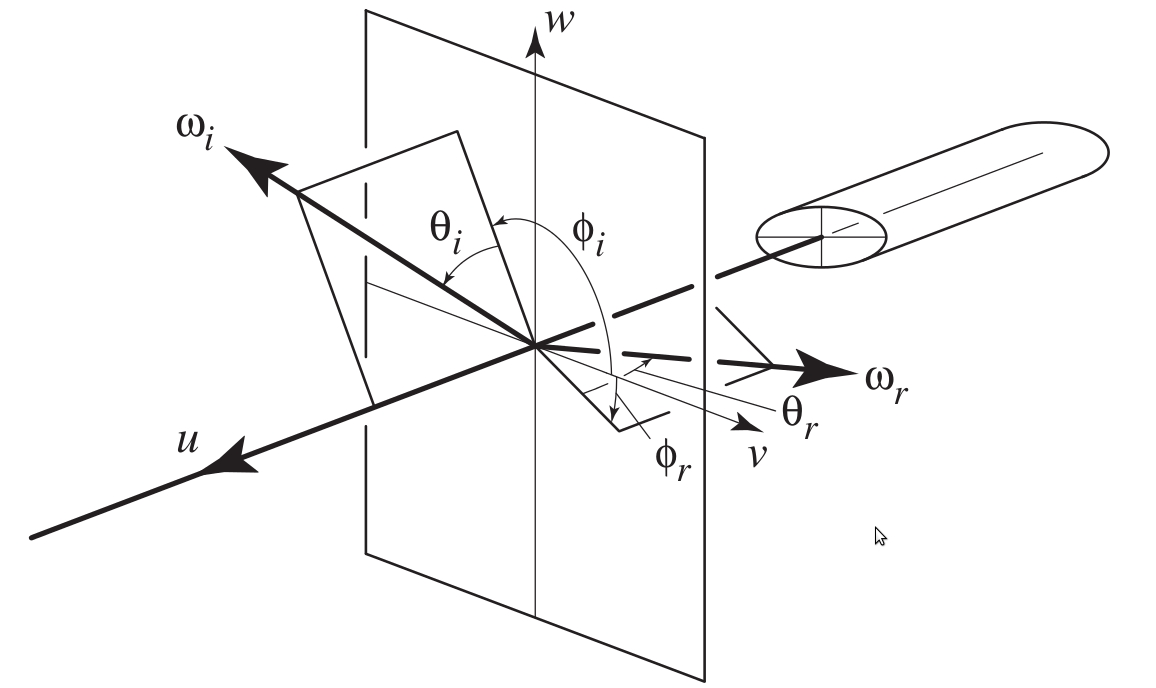
\includegraphics[scale=.4]{images/axes.jpeg}

\caption{An overview of the coordinate axes and the spherical angles with respect to a hair fiber. This is the convention used in this thesis and is used by Marschner et al. and most other hair rendering algorithms. Picture taken from Marschner et al.~\cite{marschner}.}
\label{axis_overview}

\end{figure}
\end{center}


\section{Hair Rendering Overview}

Ward et al.~\cite{ward} provides a good overview on hair rendering in general.

\subsection{Single fiber scattering}

Kajiya and Kay~\cite{kajiya} provided one of the first widely used hair scattering models that was designed to render fur. Their idea was that fine hair geometry should not be represented with complex geometry which leads to aliasing effects, but with texels. A texel is a three-dimensional texture map intended to represent a highly complex collection of surfaces contained within a defined volume~\cite{kajiya}.

The rendering of the hair model was based on a diffuse and specular component. The diffuse component is obtained by simply integrating a Lambert surface along one half of the cylinder facing the light source. The specular component is based on the Phong model in which light is reflected at a mirror angle along the tangent. Since the normals on the cylinders point in all directions perpendicular to the tangent, the reflected light forms the cone whose angle at the apex is equal to the angle of incidence~\cite{kajiya}. The Kajiya and Kay model is clearly an ad-hoc model where hair fibers are treated as opaque cylinders, limiting the realism of the model.\\

The Kajiya and Kay model lacks directionality, meaning that hairs are fully lit independent on the light direction or eye vector. Goldman~\cite{goldman} was interested in reflection and transmission and increased directionality by introducing two new attenuation factors. These attenuation factors can be used to tune the relative transmissivity and reflectivity of a hair. It does this by computing a value $f_{\textsc{dir}}$ that is multiplied with the contribution of the Kajiya and Kay model.\\

Marschner et al.~\cite{marschner} improved the Kajiya and Kay model substantially by proposing the most physically based hair scattering model at that time. Their model makes two improvements to Kajiya and Kay's model: it predicts the azimuthal variation in scattered light based on the ray optics of a cylinder, and it accounts for the longitudinal separation of the highlight into surface-reflection, transmission, and internal-reflection components that emerge at different angles~\cite{hadap}. The Marschner model is described in detail in section~\ref{sec_marschner}.


\subsection{Multiple fiber scattering}

TO DO:

Path Tracing,
Photon Mapping,
Dual Scattering Algorithm

%
% ===============================================================================
%  Marschner Model
% ===============================================================================
%

\section{Marschner model}
\label{sec_marschner}
%
% Goal of Marschner 
%

The biggest drawback of Kajiya and Kay~\cite{kajiya} is that their scattering model is not based on physical measurements. Instead, it uses a simple ad-hoc term with a constant linear highlight. Marschner et al. ~\cite{marschner} proposed a physically based scattering model for single fiber scattering. The single fiber scattering model, or Marschner model, forms the basis for the dual scattering approximation and will be discussed in detail.


\subsection{Observations}
%
% Basic observation
%
 
In order to come up with a physically based scattering model for single hair fibers, Marschner et al. devised a setup to capture the response of light scattered against a hair fiber. 

They illuminated individual hairs with a narrow beam and measured the scattered light in various directions, using a setup based on a four-axis goniometer that positioned a light source and a CCD camera at arbitrary directions from the sample~\cite{marschner}. Their measurements show a couple of distinct characteristics for human hair.

\subsubsection{Longitudinal variation}
\label{sec_longitudinal_observation}

Stamm et al. and Bustard and Smith measured the scattering behaviour in the incidence plane. This is the 2D slice for which the hair fiber is coplanar with the source and detector. Marschner et al. did the same measurements and placed a light source under a direction of positive and negative 45 degrees with the hair fiber ($\theta_i = +/- 45\degree$). See figure~\ref{fig_longitudinal_marschner} for the measured responses.

Observations show that synthetic hair has a highlight that appears exactly at the specular direction ($\theta_r = -\theta_i$), but for real hair fibers the specular highlight is shifted toward the root of the hair fiber. This is due to the tilted cuticle scales that have a surface orientation that is shifted by approximately 6 to 8 degrees from the ideal cylinder surface normal. This highlight is the result of scattering against the surface of the hair fiber. It is called the primary specular highlight and appears as having the color of the light source.

\begin{figure}[h]
\begin{center}
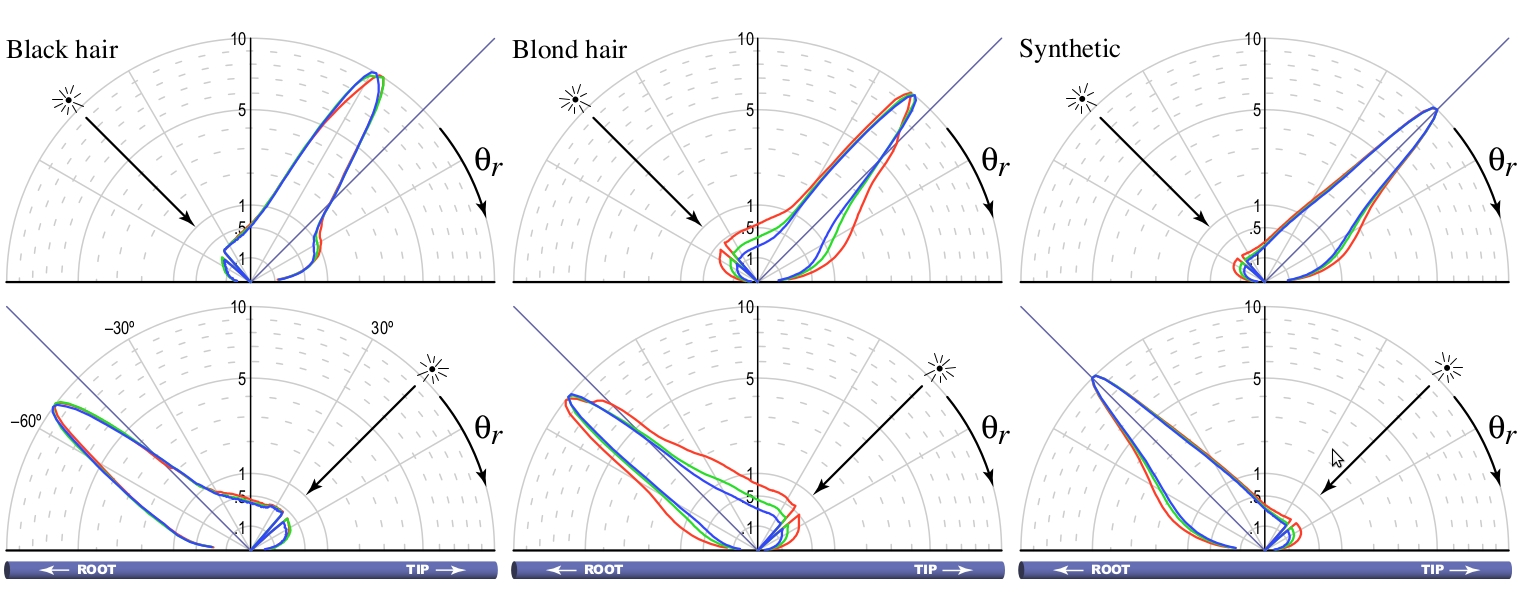
\includegraphics[scale=0.35]{images/longitudinal_response.jpeg}
\caption{The scattering behaviour in the incidence plane (longitudinal scattering). For human hair the specular reflection is shifted towards the root by a few degrees. For synthetic hair no shifted highlight is visible, because synthetic hair doesn't consist of tilted cuticle scales.}
\label{fig_longitudinal_marschner}
\end{center}
\end{figure}

Another observation is that blond hair has a coloured secondary peak. This can be seen by the red response that is slightly higher compared to the blue and red response. The secondary peak can be explained by internal scattering. Consider the hair fiber as a cylinder; when light enters the cylinder, the light will first refract, then propagates through the core of the fiber and bounces back against the other end of the fiber. When leaving the fiber, the light refracts again. This reflection and refraction behaviour causes the deviation from the primary specular highlight. During its travel, light propagated through the center of the hair fiber, where the pigments are. These pigments absorb part of the energy in different wavelengths. This is how the secondary peak gets its colour.

Furthermore, Marschner et al.~\cite{marschner} noted that as the scattering angle increases, the secondary highlight fades out, while the primary highlight maintains more constant amplitude. Both peaks maintain approximately constant width and at high angles the primary highlight becomes a sharp peak that is prominent very close to the specular direction. 


\subsubsection{Azimuthal variation}


\begin{figure}[h]
\begin{center}
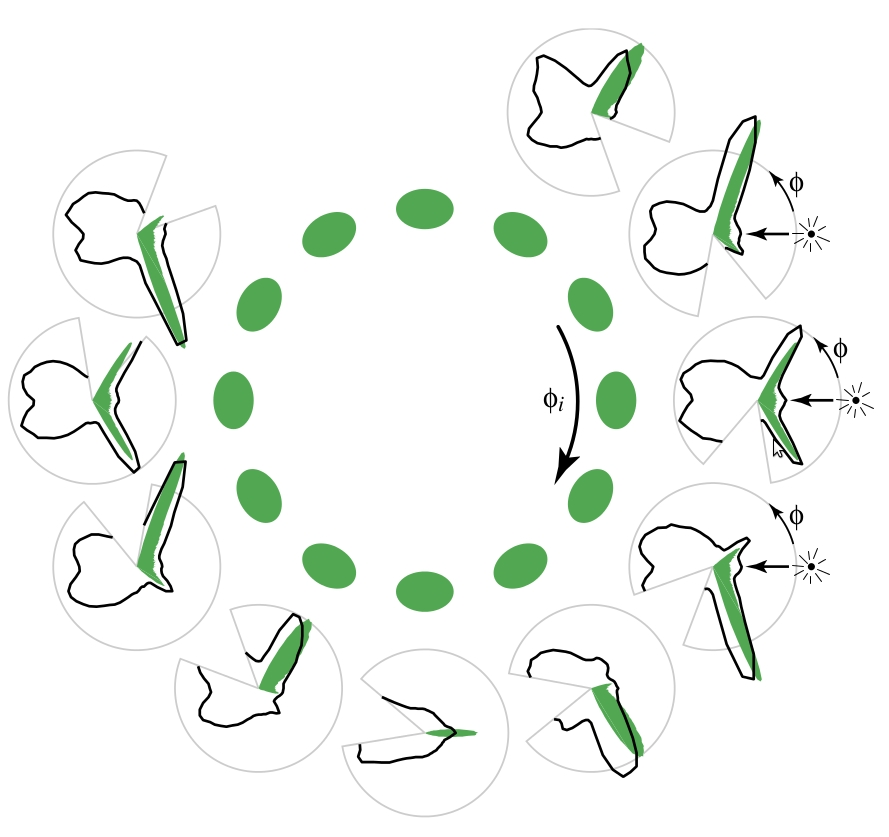
\includegraphics[scale=0.4]{images/azimuthal_measurement.jpeg}
\caption{Measurements of azimuthal scattering (scattering in the normal plane). The light source is shining from the right, while the hair fiber is rotated. The green ellipse is the cross section of the fiber for different measurements with increasing rotations of the fiber. Figure taken from Marschner et al.~\cite{marschner}.}
\label{fig_azimuthal_marschner}
\end{center}
\end{figure}


Azimuthal variation is measured by placing the light and detector in the plane that is perpendicular to the hair fiber: the normal plane. In figure~\ref{fig_azimuthal_marschner} plots are displayed that show the azimuthal scattering response with varying $\phi_i$ and $\phi_r$. The setup is that the light source is fixed (targeted from right to left) and the hair fiber is rotated. 

In this normal plane setup, it is clearly visible that there are two bright out-of-plane peaks. Out of plane, because the response is captured at $\theta_r = 10$ degrees, due to the tilted cuticle scales discussed before. These peaks are called glints.

The glints change considerably in brightness and position as a function of $\theta_i$,  meaning that the hair is not rotationally symmetric~\cite{marschner}. This is because the hair is eccentric and has an elliptical cross section. More generally, the evolution of the peaks as the fiber rotates appears similar to the internal reflection from a transparent elliptical cylinder~\cite{marschner}.

Figure~\ref{fig_azimuthal_marschner} also shows a strong transmission component. This is light that passes through the hair fiber and leaving on the other side of the fiber as seen from the light source. This means that the Marschner hair model takes three scattering modes into account. R stands for reflection and T for transmission:

\begin{itemize}
\item R: Specular reflection that is deviated slightly from the perfect specular direction, due to the cuticle scales.
\item TT: Transmission component that enters the fiber, propagates through it and leaves the fiber at the other end.
\item TRT: Internal reflection, that enters the fiber, scatters back and leaves again at the same side as where it entered.
\end{itemize}

More scattering modes are possible as well, such as TRRT or TRRRT. These events are ignored, because their contributions become negligible small due to loss of energy after that many reflection events. Instead, Marschner et al.~\cite{marschner} suggests to add a little diffuse color for better looking results. In figure~\ref{female_hair} an image is shown with the three scattering components clearly visible.

\begin{figure}[h]
\begin{center}
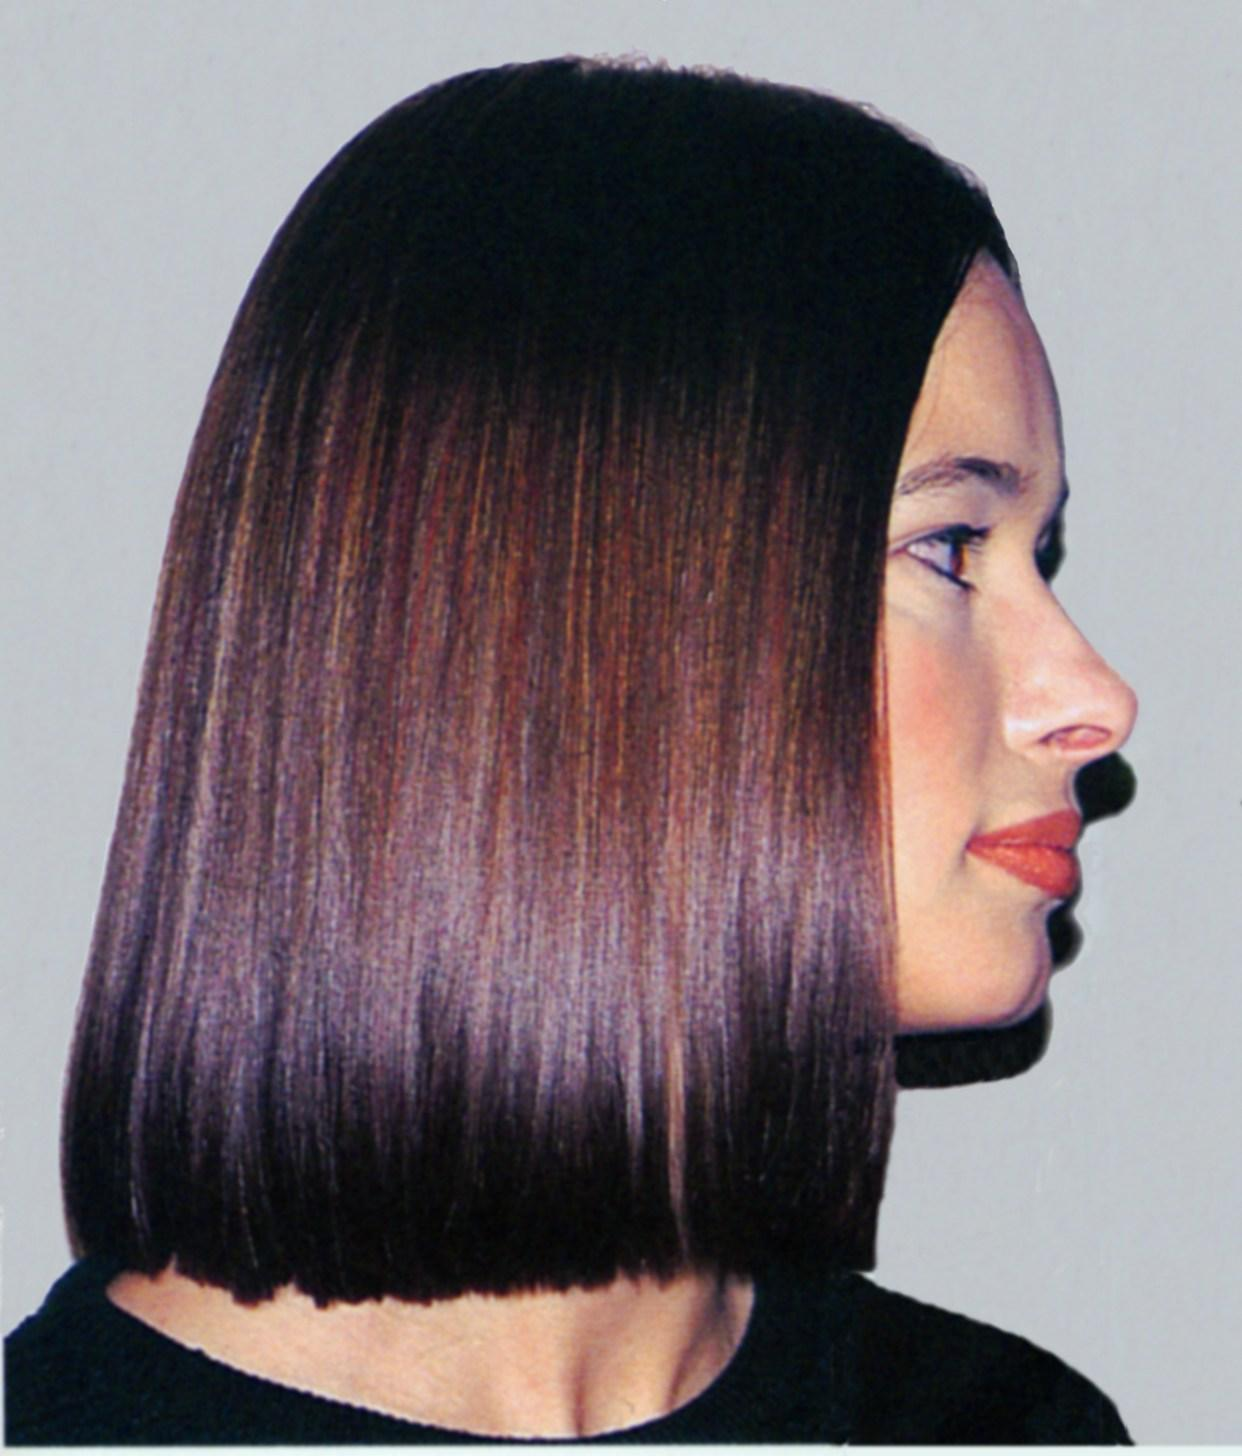
\includegraphics[scale=0.2]{images/female_marschner.jpeg}
\caption{An image from Gray~\cite{gray} showing a female with brown hair. The three scattering modes: R, TT and TRT contributions are visible in the hair. Glints give hair it's characteristic texture.}
\label{female_hair}
\end{center}
\end{figure}

\subsection{Model}

There are properties that have been used in previous work on scattering from fibers ([Marcuse 1974; Adler et al. 1998; Mount et al. 1998]):

\begin{itemize}
\item A ray that enters a dielectric cylinder at a particular angle to the axis will always exit at the same angle, regardless of the sequence of reflections and refractions it undergoes.

\item The dependence of the scattered distribution can be analysed by examining only the projection into a plane perpendicular to the hair.
\end{itemize}

Based on the observations described in the previous subsection and the theory here, Marschner et al. came up with a model that is divided into a longitudinal scattering component $M$ and an azimuthal scattering component $N$. Each scattering mode (R, TT and TRT) has it's own component, resulting in the following scattering model:

\begin{equation}
S(\omega_i, \omega_r) = M_r
\end{equation}

$S$ depends on incoming and outgoing angles $\omega_i$ and $\omega_r$, but can be reduced to a 2D scattering function, since the scattering model makes use of the difference angles $\theta_h$ and $\phi$.

\subsubsection{Longitudinal Scattering Function}

Using the first property of scattering from fibers, it can be derived that the angle of incidence will be the same as the angle of reflection ($\theta_i = -\theta_r$). There are two deviations that cause the reflection to not be exactly in the specular direction (see section~\ref{sec_longitudinal_observation}). First, the surface of hair fibers are rough, causing a spread of reflected light instead of a mirror reflection. Secondly, the cuticle scales of the hair fiber cause a 6 to 8 degrees deviation from the perfect specular direction.

Marschner et al. approximated the longitudinal scattering function $M$ by a unit-integral zero-mean Gaussian function $g(\beta, x)$, where $\beta$ equals the standard deviation.

The resulting longitudinal scattering functions are displayed in figure~\ref{longitudinal_marschner}.

\begin{figure}
\begin{gather*}
M_R(\theta_h) = g(\beta_R, \theta_h - \alpha_R) \\
M_{TT}(\theta_h) = g(\beta_{TT}, \theta_h - \alpha_{TT}) \\
M_{TRT}(\theta_h) = g(\beta_{TRT}, \theta_h - \alpha_{TRT})
\end{gather*}

\caption{Longitudinal scattering functions for the Marschner model.}
\label{longitudinal_marschner}
\end{figure}

By varying the standard deviation $\beta$, the spread of the longitudinal scattering component can be adjusted to simulate the rough surface of hair fibers. $\alpha$ deviates the peak from the specular direction by shifting the gaussian distribution. Marschner et al~\cite{marschner} provided some typical values for $\alpha$ and $\beta$ (see table~\ref{table_marschner_alpha_beta}).

\begin{table}[h]
\begin{tabular}{c|l|c}
Parameter & Description & Typical value \\ \hline 
$\alpha_{R}$ & Longitudinal shift for R lobe & -10\textdegree\,to -5\textdegree \\
$\alpha_{TT}$ & Longitudinal shift for TT lobe & $-\alpha_R / 2$ \\
$\alpha_{TRT}$ & Longitudinal shift for TRTlobe & $-3\alpha_R / 2$ \\
$\beta_R$ & Longitudinal spread for R lobe & 5\textdegree\, to 10\textdegree\, \\
$\beta_{TT}$ & Longitudinal spread for TT lobe & $\beta_R / 2$ \\
$\beta_{TRT}$ & Longitudinal spread for TRT lobe & $2 \beta_R$ 
\end{tabular}

\caption{Typical values for parameters for the longitudinal scattering function. Taken from Marschner et al.~\cite{marschner}}
\label{table_marschner_alpha_beta}
\end{table}


\subsubsection{Azimuthal scattering Function}

The azimuthal scattering component requires more thought, since different scattering paths inside the circular cross section need to be considered. 

Scattering from a dielectric circle is well studied. Consider a parallel beam incident on a circular cross section at an offset $h$ from the center. A parallel beam incident on the center of a circle means that $h = 0$. A value of $h=+/-1$ indicates that the parallel beam is glancing the edges of the circle. Using the offset $h$, the angle of incidence $\gamma_i$ can be computed using the following equation:

\begin{eqnarray*}
\sin \gamma_i = h & \Leftrightarrow & \gamma_i = \arcsin h \\
\eta \sin \gamma_t = h & \Leftrightarrow & \gamma_t = (\arcsin h) / \eta
\end{eqnarray*}

A ray that is incident on the unit circle can be traced as it refracts and reflects through the circle. The exit angle is not only dependent on the incidence angle (or offset from the center), but also on the number of scattering events. The number of scattering events $p$ equals 1 for the reflection case, 2 for transmission (TT) and 3 for internal reflection (TRT). The exit angle can then be calculated as follows:

\begin{equation}
\phi(p,h) = 2p \gamma_t - 2 \gamma_i + p \pi
\end{equation}

The figure from Marschner et al. provides a good overview on the possible scattering events and the relation between the scattering angles.

Consider rendering a scene using ray tracing and that a particular camera ray is incident on a hair fiber. To find the contribution for the rendered image, we need to find all the paths that contribute to scattering in the direction of the camera ray. These paths are found by solving for roots. The R and TT cases have exactly one root and TRT has either one or three roots. The $h$ values for these paths are found by solving for the roots of the function $\phi(p, h) - \phi = 0$. Finding the roots requires solving a cubic equation, which is explained deeper in Marschner et al.~\cite{marschner}. The roots are denoted by $h(p, r, \phi)$ where different values of $r$ denote different roots. \\


Attenuation has to be taken into account as well. Attenuation occurs because of reflections, refractions and absorption. The attenuation for reflections and refractions are computed using the Fresnel equation. The Fresnel equation takes a parallel and perpendicular index of refraction ($\eta'$ and $\eta''$ respectively). Absorption takes place when a ray propagates through the hair fiber. The length of each internal path segment is computed by applying the law of cosines. According to~\cite{}, the formula given in Marschner et al. is wrong. This equation should be as followed:

\begin{equation}
l = \frac{2r \cos \gamma_t}{\cos \theta_t}\,\,\, \textsf{with $\theta_t = -sgn(\theta_i) \arccos ((\eta'' / \eta') \cos \theta_i)$}
\end{equation}

Here $l$ denotes the length of a single internal path segment for the TT case. For TRT, the length doubles. $r$ is the radius of the hair fiber and is a setting provided by the user. Absorption is denoted by $T(\sigma_a, h)$ where $\sigma_a$ is the absorption coefficient. It describes the amount of absorption per unit length through the hair fiber. It follows straightforwardly that the absorption is computed as $T(\sigma_a, h) = \exp( \sigma_a l )$. The normal plane scattering function $N_p$ can now be described and is shown in equation~\ref{azimuthal_marschner} be described.

\begin{eqnarray*}
A(0, h) & = & \textrm{Fresnel}( \eta', \eta'', \gamma_i ) \\
A(p, h) & = & (1 - \textrm{Fresnel}( \eta', \eta'', \gamma_i ))^2 \cdot \textrm{Fresnel}( \frac{1}{\eta'}, \frac{1}{\eta''}, \gamma_t )^ {p-1} \cdot T(\sigma_a, h) \\
\label{azimuthal_marschner}
\end{eqnarray*}

The normal plane scattering function for a given number of path segments $p$ (1, 2 or 3) is given in equation~\ref{azimuthal_marschner}.

\begin{equation}
N_p(p, \phi) = \sum\limits_r A(p, h(p, r, \phi)) \cdot \Big \vert 2 \frac{d\phi}{dh}( p, h(p, r, \phi) ) \Big \vert^{-1}
\end{equation}

\subsubsection{Glints}

Because the theory is based on smooth surfaces, the normal plane scattering function $N_p$ for the TRT scenario produces singularities with infinite intensity~\cite{marschner}. These caustics are removed by replacing it with a smooth Gaussian lobe centered at the location of the caustic. This changes the normal plane scattering function for the TRT case. Marschner et al.\cite{marschner} provides more detail into how the scattering function changes.

\subsubsection{Taking into account eccentricity}

Changing refractive index has effects that are qualitatively similar to changing eccentricity~\cite{marschner}. In order to simulate eccentricity, the refractive index is computed based on the value of eccentricity $a$. The equation can be found below. More detail is in Marschner et al's paper~\cite{marschner}.

\begin{eqnarray}
\eta_1^* & = & 2(\eta - 1) a^2 - \eta + 2 \\
\eta_2^* & = & 2(\eta - 1) a^{-2} - \eta + 2 \\
\eta^*(\phi_h) & = & \frac{1}{2}\big((\eta_1^* + \eta_2^*)+\cos(2\phi_h)(\eta_1^* + \eta_2^*) \big)
\end{eqnarray}

\subsubsection{Marschner model}

From the description above we can now describe the complete Marschner scattering model $S(\omega_i, \omega_r)$.

\begin{eqnarray*}
S(\phi_i,\theta_i; \phi_r, \theta_r) & = & M_R(\theta_h) N_R(\phi) / \cos^2 \theta_d \\
& + & M_{TT}(\theta_h) N_{TT}(\phi) / \cos^2 \theta_d \\
& + & M_{TRT}(\theta_h) N_{TRT}(\phi) / \cos^2 \theta_d \\
\end{eqnarray*}

Here the longitudinal functions $N_x$ are placeholders for the normal plane scattering function $N_p$:

\begin{eqnarray*}
N_R(\phi) & = & N_p(0, \phi) \\
N_{TT}(\phi) & = & N_p(1, \phi) \\
N_{TRT}(\phi) & = & N_p(2, \phi) \\
\end{eqnarray*}
\subsection{Evaluation}

The advantage of the Marschner hair model is that it is based on physical observations. Compared to previous approaches this is a huge win. Finding the roots for a given direction is slow, but can be dealt with by using precomputed tables.

The Marschner hair model focuses on single fiber scattering and to render realistic hair volumes, multiple fiber scattering needs to be taken into account. Path tracing or photon mapping are possible approaches, but take a lot of time or require an extensive amount of memory. Another drawback is that from own calculations, the Marschner model is not energy conserving. Especially for very wide angles, the reflections will be relatively high.

%
% ===============================================================================
%  Dual Scattering
% ===============================================================================
%

\section{Dual Scattering}

The dual scattering model builds on top of Marschner. Marschner simulated the appearance of scattering effects for a single hair fiber. To render a full human head consisting of many hair strands, path tracing or any other form of tracing light through a volume should be considered to accumulate the effects of single fiber scattering. Multiple fiber scattering is obviously more complex and some approximation strategies are helpful to speed up the rendering. Most approximation techniques so far are too coarse and do not look close to path tracing results. The Dual Scattering Approximation method for rendering multiple fiber scattering does a great job at coming close to path tracing results while still having an efficient algorithm.

\subsection{Theory}

\subsection{Evaluation}



%
% ===============================================================================
%  Importance sampling
% ===============================================================================
%

\chapter{Approach}

In this thesis project, the goal is to extend the dual scattering approximation with importance sampling. As explained in section~\ref{} importance sampling is a variance reduction technique by taking into account the samples that contribute the most to the final image.

There are a couple of observations to be made for the dual scattering approximation model. First, there is a difference between direct reflection for light that is scattered one or multiple times through the hair volume.

As light scatters through the hair volume, the spread becomes isotropic after only a few scattering events. See images below.

\section{Observations}

The images in figure~\ref{visual_light_distribution} show the scattering distribution for hair fibers that are directly hit by light rays (left) and hair fibers where the light has scattered through other fibers first (right). This difference is important,  because the dual scattering algorithm approximates global scattering based on the number of hair strands the light ray has passed through. Hair fibers at the boundary are most likely hit directly by light rays (if the light source is on the same side of the hair volume). Light rays scattering through fibers inside the hair volume, will likely scatter through other fibers first before arriving at the fiber in question.

A couple of observations can be made.
\begin{itemize}
\item Hair fibers that are directly hit by the light source have a strong transmission component. This comes from the fact that it is essentially single fiber scattering, and therefore resembles the Marschner model.
\item Scattering for fibers inside the hair volume, or fibers for which the light ray has scattered through one or multiple fibers, show a remarkable amount of uniform scattering.
\end{itemize}

\section{Importance Sampling Function}

The scattering behaviour is dependent on two parameters: $\theta$ and $\phi$. The relationship between the two are important in finding an importance sampling function.

In figure~\ref{spherical_plot} the response is shown for 


 The left images shows the distribution for hair fibers that are directly hit by the light.  This happens for hair fibers at the boundary of the hair volume (i.e. direct scattering). The right image shows the scattering distribution for a hair strand situated in the hair volume. No scattering.


\begin{figure}
\begin{tabular}{c}
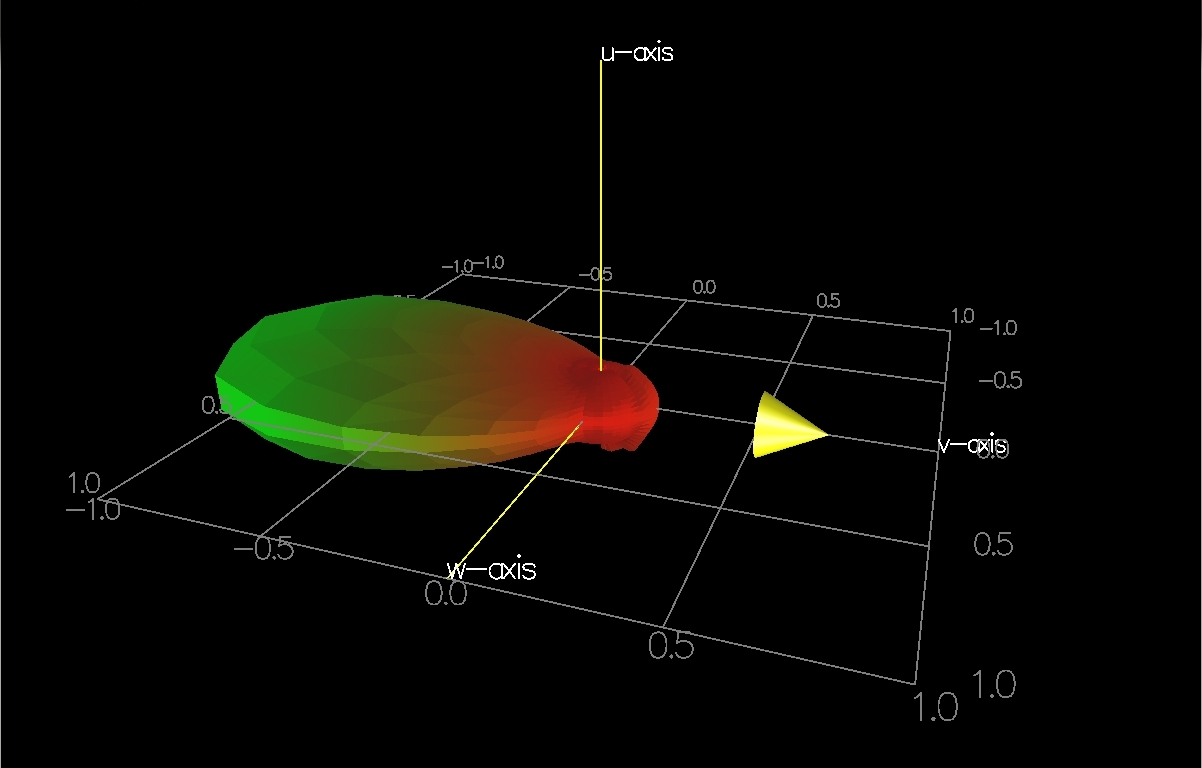
\includegraphics[scale=0.2]{images/strands0_colorR.jpg}
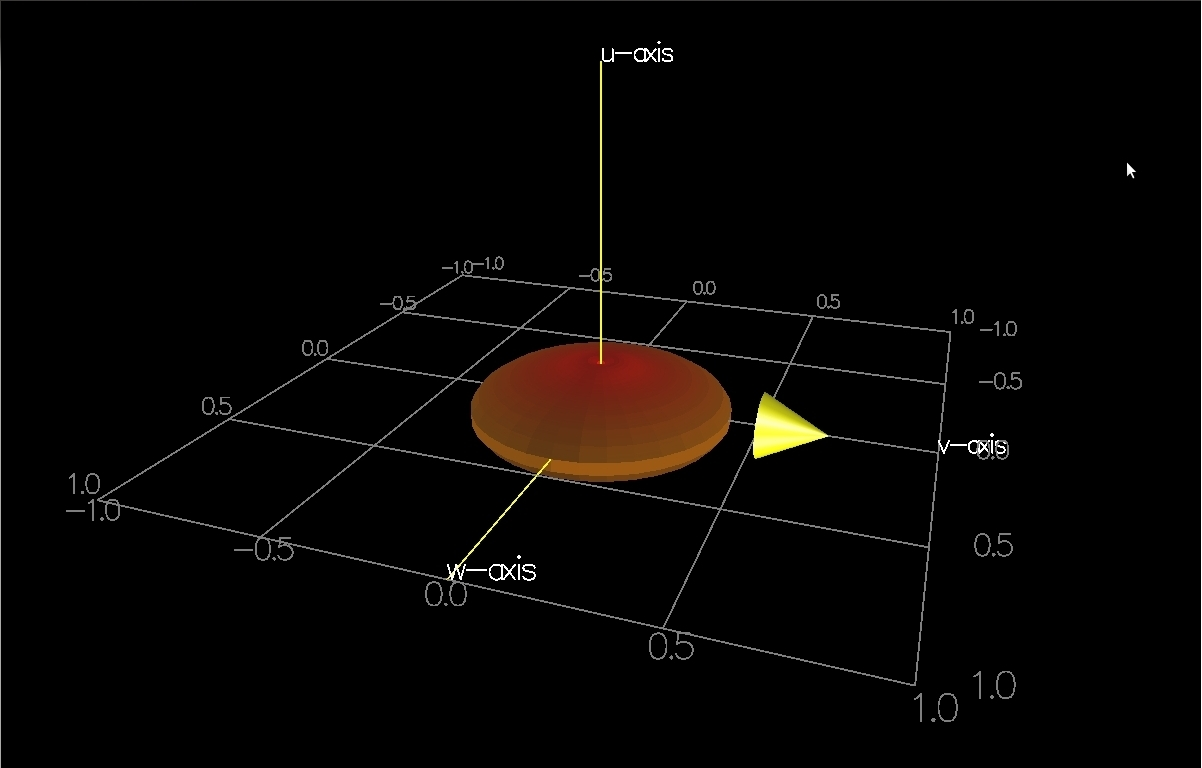
\includegraphics[scale=0.2]{images/strands1_colorR.jpg} \\
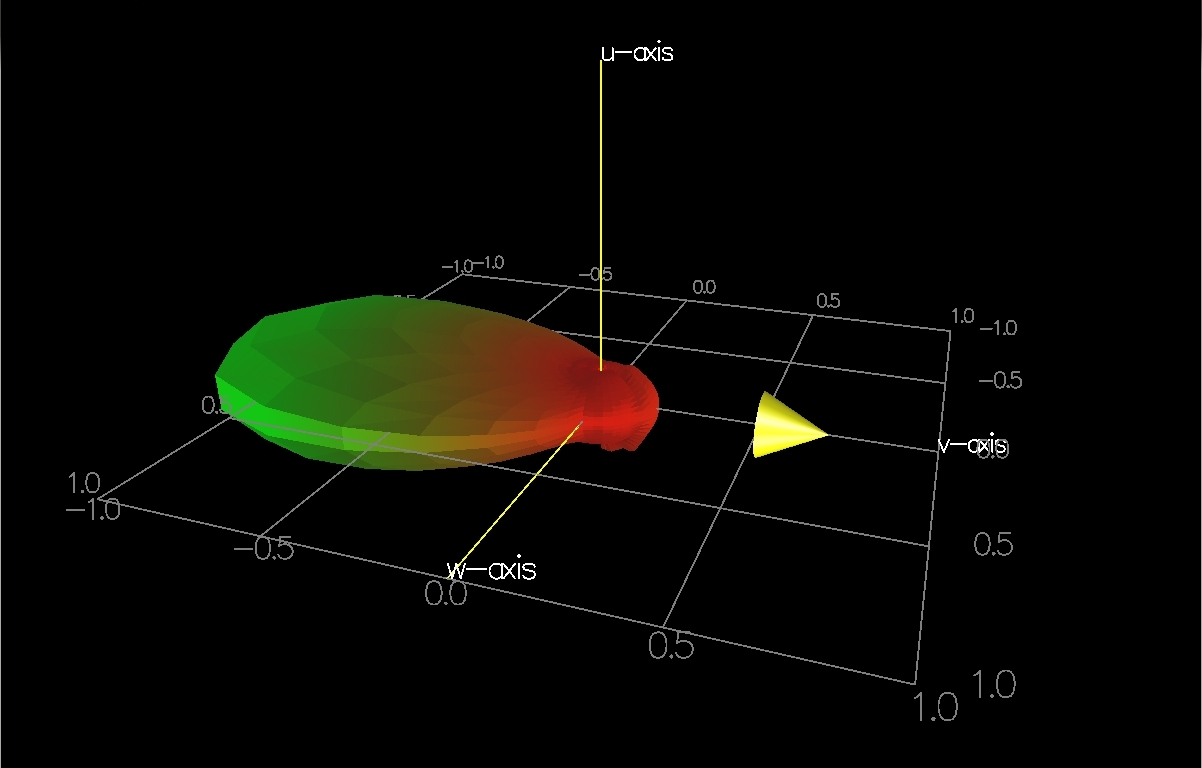
\includegraphics[scale=0.2]{images/strands0_colorR.jpg}
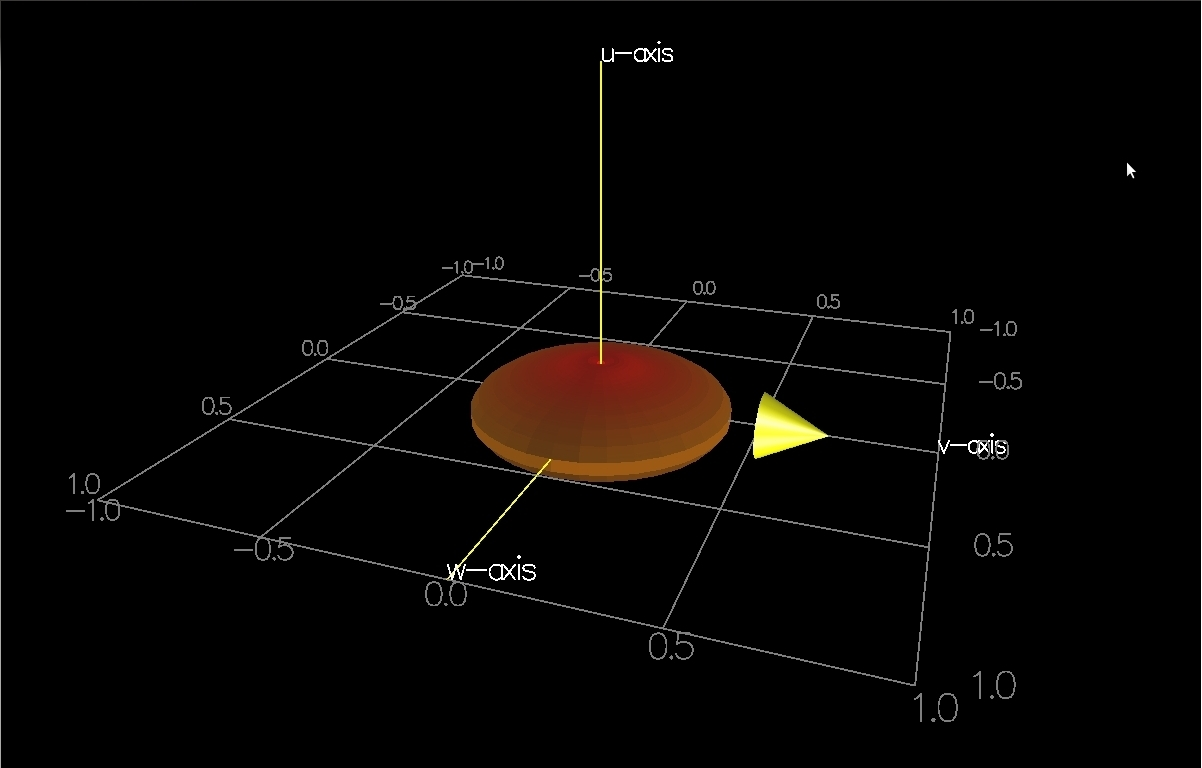
\includegraphics[scale=0.2]{images/strands1_colorR.jpg} \\
\end{tabular}

\caption{Distribution of light when scattered against a hair fiber. The hair fiber runs along the u-axis and light is coming from the light source, depicted as the yellow cone.}
\label{visual_light_distribution}

\end{figure}



A detailed description of the contributions in this project


\begin{figure}
\begin{tabular}{c}
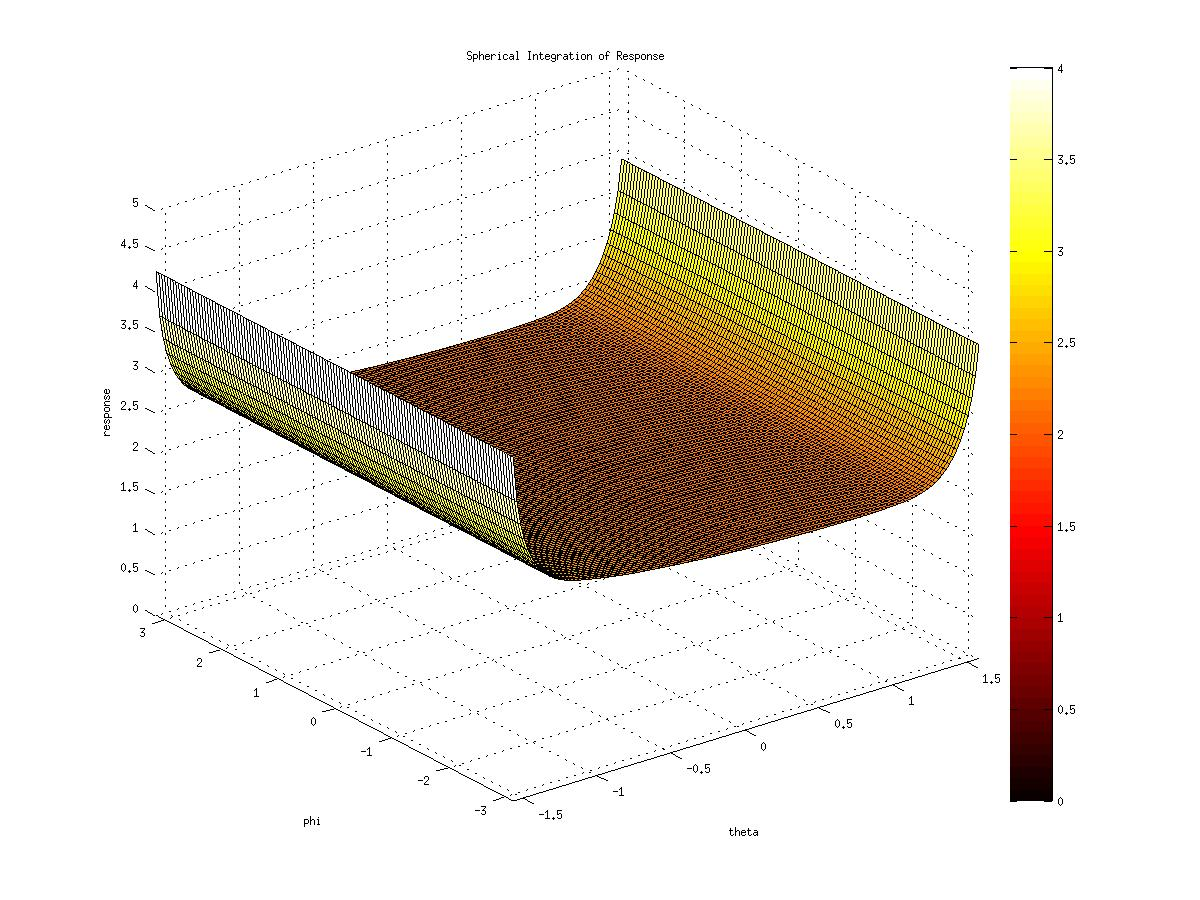
\includegraphics[scale=0.3]{images/plots/sphericalintegration_dualscattering_00.jpg} \\

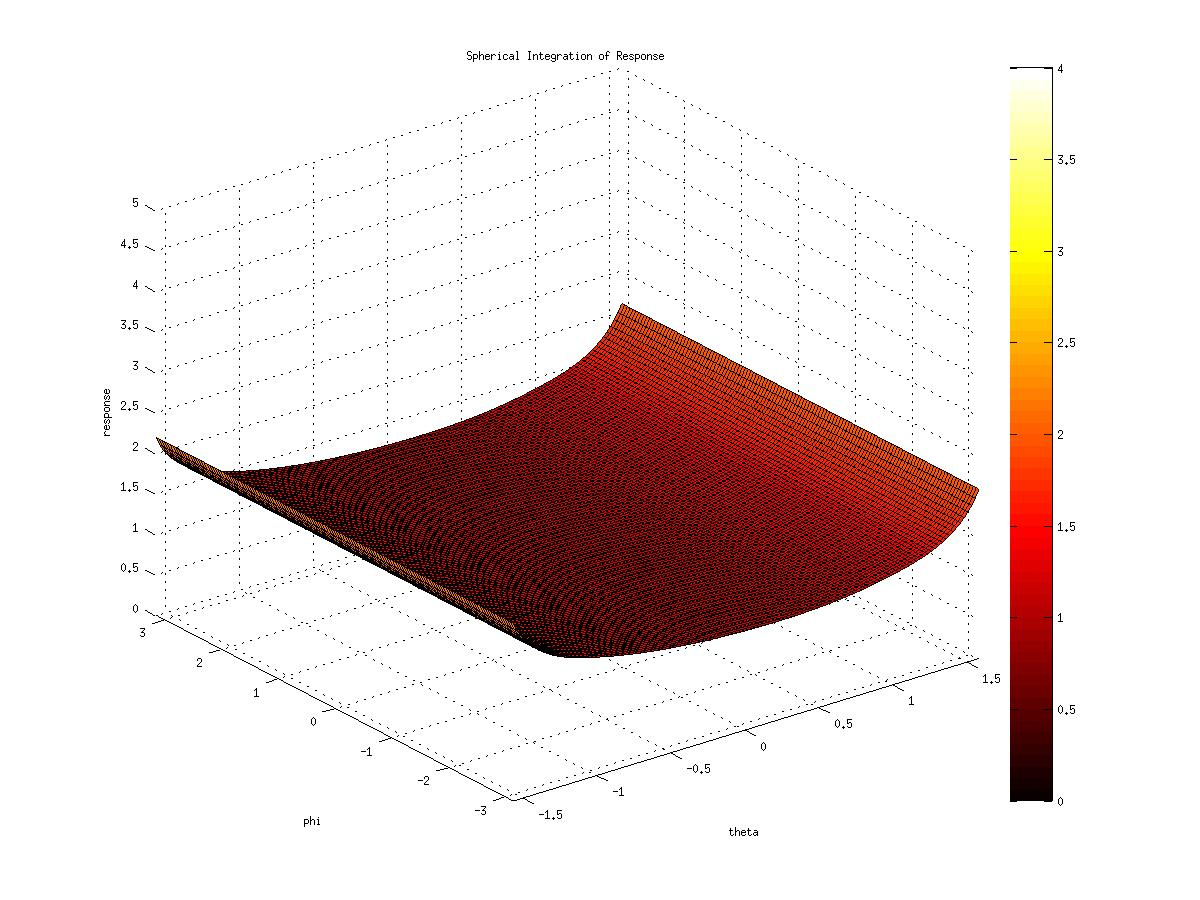
\includegraphics[scale=0.3]{images/plots/sphericalintegration_dualscattering_01.jpg} \\


\caption{Distribution of light when scattered against a hair fiber. The hair fiber runs along the u-axis and light is coming from the light source, depicted as the yellow cone.}
\label{visual_light_distribution}

\end{figure}

\section{Importance Sampling}
The Marschner model is a physically based algorithm, but it is not energy conserving. Enforcing approximate energy conservation at grazing angles can be performed by clamping and simplifying the weight of the Monte Carlo estimator, as has been explained by~\cite{hery}.

Box Muller Transform

The importance sampling idea in dual scattering consists of two ideas. Considering a point on the hair model. It can either have an unobstructed path to the light source, or it can have hair strands in between covering the point from the light source.

\section{Analyzing Graph response for Dual scattering model}

The response of the dual scattering approximation function depends on numerous parameters. To efficiently importance sample the dual scattering algorithm, we need to take these variations into account.

The parameters that have a considerable impact on the graph response are:
\begin{itemize}
\item The shape of the cross section eccentricity value
\item The number of hair strands between the shading point and light source: $n$
\end{itemize}

\section{}
Importance sampling is a strategy to reduce the variance, by generating samples that , as has been explained in section~\label{importance_sampling},

\section{Cauchy}

To extend the strategy with importance sampling, we need to find a sampling function that closely matches the response from the graphs in the previous section.


The dual scattering approximation To importance samp


\chapter{Results}

\section{Evaluation Strategy}

Experimental Results plus evaluation

\chapter{Conclusion}

\chapter{Appendix}

\bibliography{thesis}
\bibliographystyle{plain}

\end{document}
